% Template for ICME-2013 paper; to be used with:
%          spconf.sty  - ICASSP/ICIP LaTeX style file, and
%          IEEEbib.bst - IEEE bibliography style file.
% --------------------------------------------------------------------------
\documentclass{article}
\usepackage{spconf,amsmath,epsfig}

\usepackage[utf8]{inputenc}

\usepackage{subfig}
\usepackage{enumerate}

% autoref command
\usepackage[hyphens]{url}
\usepackage[pdftex,urlcolor=black,colorlinks=true,linkcolor=black,citecolor=black]{hyperref}
\def\sectionautorefname{Section}
\def\subsectionautorefname{Subsection}
\def\subfigureautorefname{Subfigure}

% listings and Verbatim environment
\usepackage{fancyvrb}
\usepackage{relsize}
\usepackage{listings}
\usepackage{verbatim}
\newcommand{\defaultlistingsize}{\fontsize{8pt}{9.5pt}}
\newcommand{\inlinelistingsize}{\fontsize{8pt}{11pt}}
\newcommand{\smalllistingsize}{\fontsize{7.5pt}{9.5pt}}
\newcommand{\listingsize}{\defaultlistingsize}
\RecustomVerbatimCommand{\Verb}{Verb}{fontsize=\inlinelistingsize}
\RecustomVerbatimEnvironment{Verbatim}{Verbatim}{fontsize=\defaultlistingsize}
\lstset{frame=lines,captionpos=b,numberbychapter=false,escapechar=§,
        aboveskip=2em,belowskip=1em,abovecaptionskip=0.5em,belowcaptionskip=0.5em,
        framexbottommargin=-1em,basicstyle=\ttfamily\listingsize\selectfont}

\pagestyle{empty}

\begin{document}\sloppy

% for 1st, 2nd, etc. superscripting
\newcommand{\ts}{\textsuperscript}

% Title.
% ------
\title{Tell me why! Ain't nothin' but a~mistake?\\ Describing Media Item Differences with Media Fragments URI}
%
% Single address.
% ---------------
\name{Anonymous ICME submission}
\address{}

\maketitle

%
\begin{abstract}
We have developed a~tile-wise histogram-based
media item deduplication and clustering algorithm
with additional high-level semantic matching criteria
that is tailored to photos and videos stemming from multiple social networks.
In this paper, we investigate whether the addressing scheme
Media Fragments {\sc uri} provides a~feasible and practicable way
to vividly and graphically describe media item differences
between media items of type photo and/or video.
\end{abstract}
%
\begin{keywords}
Media Fragments {\sc uri}, Media Fragments, Media Items, Deduplication, Social Networks
\end{keywords}
%
\section{Introduction}
\label{sec:introduction}

The \emph{Backstreet Boys}~({\sc bsb}) are a~boy band
formed in~1993 in Orlando,~FL
that have sold over 130~million records worldwide,
making them the best-selling boy band of all time.
In~2013, the band will celebrate their 20\ts{th}~anniversary
with a~new album and a~world tour.
Reason enough for us to make them titular saint of this paper
with their hit song \emph{I~Want It That Way}
from the album \emph{Millennium}.
While the spike of their career was in the late 90s,
even today people still actively share,%
\footnote{{\sc bsb} on social networks: \url{http://bit.ly/backstreet-gplus}
and \url{http://bit.ly/backstreet-fb},
both accessed 03/04/2013}
publish, and follow the group on \emph{social networks}.

\subsection{Previous Work}
\label{sec:previous-work}

Social networks are at the heart of our research on event summarization,
specifically deduplicating \emph{exact-} and \emph{near-duplicate}
media items that optionally accompany textual status messages
referred to as \emph{microposts} on multiple social networks. 
In the context of our research, we define a~\emph{media item}
as either a~photo (image) or video
that was \emph{publicly} shared or published
on at least one social network.
\autoref{fig:near-duplicate} shows an example
where two users of the social networks Facebook and Google+
independently of each other share a~\emph{near-duplicate} media item
in form of the music video \emph{Everybody}
performed by the \emph{Backstreet Boys}.
In order to detect, deduplicate, and cluster such occurrences
of \emph{exact-} and \emph{near-duplicate}
media items being shared independently across social networks,
we have implemented a~tile-wise histogram-based algorithm
with additional high-level semantic matching criteria
that was shown to work effectively and efficiently for several events.

\begin{figure}[b!]
  \centering
  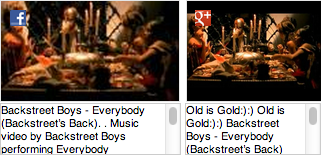
\includegraphics[width=1\linewidth]{./backstreetboys.png}
  %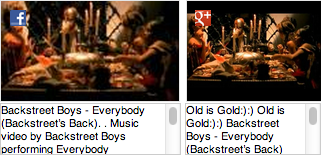
\includegraphics[width=0.796\linewidth]{./backstreetboys.png}  
  \caption{\emph{Near-duplicate} music video \emph{Everybody}
    by the \emph{Backstreet Boys} shared
    independently on Facebook and Google+}
  \label{fig:near-duplicate}
\end{figure}

\subsection{Motivation and Research Question}
\label{sec:motivation-and-research-question}

During previous experiments on deduplicating event-related media items,
we noticed that human raters wanted to know \emph{why}%
\footnote{Tell me why! Ain't nothin' but a~mistake?}
certain media items were clustered as \emph{exact-} or \emph{near-duplicates}.
In consequence, in this paper, we investigate in how far
Media Fragments {\sc uri}~\cite{troncy2012mediafragments}
provides a~feasible and practicable way
to tell raters why media items were clustered.
As we deal with media items of type photo and/or video,
we make simultaneous use of two types of media fragments dimensions,
the temporal dimension and the spatial dimension.

\subsection{Paper Structure}
\label{sec:paper-structure}

The remainder of this paper is structured as follows.
In \autoref{sec:related-work}, we report on related work
on media fragments, digital storytelling, and natural language generation.
In \autoref{sec:media-fragment-requirements}, we describe
our requirements on media fragments identifiers.
In \autoref{sec:media-item-deduplication-algorithm},
we detail how the media item deduplication algorithm works
and show low-level debugging approaches to check
\emph{if} or \emph{if not} media items are clustered.
In \autoref{sec:from-debug-output-to-story},
we elaborate on how this low-level debug output gets lifted
to natural language stories for human raters to understand
\emph{why} or \emph{why not} media items are clustered.
The chosen approach gets evaluated in \autoref{sec:evaluation}.
We conclude in \autoref{sec:conclusions-and-future-work}
and give an outlook on future work.

\section{Related Work}
\label{sec:related-work}

\noindent \textit{Media Fragments:}
There are many online video hosting platforms
that have some sort of media fragments support.
In the following, we present two representative ones.
The video hosting platform YouTube%
\footnote{YouTube: \url{http://www.youtube.com/}}
allows for deep-linking into videos
via a~proprietary {\sc url} parameter \texttt{t},
whose value has to match the regular expression
\texttt{\textbackslash d+m\textbackslash d+s} (for minutes and seconds),
as documented in~\cite{youtube2008link}.
Dailymotion\footnote{Dailymotion: \url{http://www.dailymotion.com/}}
has a~similar, albeit undocumented, {\sc url} parameter \texttt{start},
whose value has to match the regular expression
\texttt{\textbackslash d+} (for seconds).
The {\sc css} Backgrounds and Borders Module Level~3 specification~\cite{bos2012css3}
defines the \texttt{background-size} property
that---combined with a wrapping element---%
can be used to crop media items visually
and thus create the illusion of a~spatial media fragment.
Media Fragments {\sc uri}~\cite{troncy2012mediafragments} specifies
a~syntax for constructing media fragments {\sc uri}s
and explains how to handle them
when used over the {\sc http} protocol~\cite{fielding1999http}.
The syntax is based on the specification of particular name-value pairs
that can be used in {\sc uri} query strings and {\sc uri} fragment identifiers
to restrict a~media resource to a~certain fragment.
Currently supported Media Fragments {\sc uri}s %in the basic version
cover the temporal and the spatial dimension.
%The temporal dimension denotes a~specific time range in the original media,
%such as ``starting at second 10, ending at second 20.''
%The spatial dimension denotes a~specific range of pixels in the original media,
%such as ``a~rectangle of size $ 100 \times 100 $ pixels
%with its top-left at the pixel coordinates $ (10, 10) $.''
Combinations of dimensions are possible.
%as well as combining Media Fragments {\sc uri} query strings
%and {\sc uri} fragment identifiers.

\noindent \textit{Digital Storytelling:}
Pizzi and Cavazza report in~\cite{pizzi2008debugging} on the development of
an authoring technology on top of an interactive storytelling system
that originated as a~debugging%
\footnote{Note, Pizzi and Cavazza use the term \emph{debugging} in the non-IT sense:
to check for redundancy, dead-ends, consistency, \emph{etc.} in authored stories}
tool for a~planning system.
Alexander and Levine define in~\cite{alexander2008storytelling}
the term \emph{Web~2.0 storytelling}, where people create \emph{microcontent}---%
small chunks of content, with each chunk conveying a~primary idea or concept---%
that gets combined with social media to form coherent stories.
We use Media Fragments {\sc uri}s to help raters understand
the results of an algorithm by converting dry software debugging data
to digital stories.

\noindent \textit{Natural Language Generation:}
Natural language generation is the natural language processing task
of generating natural language from a~machine representation system.
The field is covered in great detail
by Reiter and Dale in~\cite{reiter2000building}.
They divide the task into three stages:
document planning, microplanning, and realization.
\emph{Document planning} determines the content and structure of a~document.
\emph{Microplanning} decides which words, syntactic structures, \emph{etc.}
will be used to communicate the chosen content and structure.
\emph{Realization} maps the abstract representations
used by microplanning into actual text.

\begin{lstlisting}[caption={Description of two 10~sec long media fragments:
  \textit{(i)}~a~tile of dimensions $ 30 \times 40 $ pixels
  starting at pixel coordinates $ (0, 0) $
  that contains a~face; and
  \textit{(ii)}~a~tile of dimensions $ 10 \times 10 $ pixels
  starting at pixel coordinates $ (0, 0) $ of red color},
  label=code:media-fragment, float=b!]
@base <http://example.org/> .
@prefix ma: <http://www.w3.org/ns/ma-ont> .
@prefix foaf: <http://xmlns.com/foaf/0.1/> .
@prefix db: <http://dbpedia.org/resource/> .
@prefix dbo: <http://dbpedia.org/ontology/> .
@prefix col: <http://purl.org/colors/rgb/> .

<video> a ma:MediaResource .

<video#t=,10&xywh=0,0,30,40> a ma:MediaFragment ;
                             foaf:depicts db:Face .
                             
<video#t=,10&xywh=0,0,10,10> a ma:MediaFragment ;
                             dbo:colour col:f00 .
\end{lstlisting}

\section{Media Fragments Requirements}
\label{sec:media-fragment-requirements}

In the context of our research on media item deduplication and clustering,
media fragments identifiers need to be capable of expressing the following concepts.

\begin{enumerate}[i]
  \itemsep0em 
  \item Given a~rectangular media item with the dimensions $ width \times height $,
    express that in turn rectangular tiles
    of smaller dimensions are part of the original media item.
  \item Given detected faces at the granularity level of bounding rectangles,
    express that these bounding rectangles are within the dimensions
    of the original media item and that each bounding rectangle contains a~face.
  \item Requirements \textit{i} and \textit{ii} need to be fulfilled for both
    types of media items, photos and videos;
    where in case of the latter, video subsegments of any length---%
    including video still frames---need to be supported.
\end{enumerate}

Media Fragments {\sc uri}~\cite{troncy2012mediafragments} as described in
the basic version of the specification supports all three requirements.
The \emph{temporal dimension} is denoted by the parameter name \texttt{t}
and specified as an interval with a~begin time and an end time.
Either one or both parameters may be omitted,
with the begin time defaulting to 0 seconds
and the end time defaulting to the duration of the source media item.
The interval is half-open: the begin time is considered part of the interval,
whereas the end time is considered to be the first time point
that is not part of the interval.
If only a~single value is present, it corresponds to the begin time,
except for when it is preceded by a~comma, which indicates the end time.
The temporal dimension is specified as Normal Play Time ({\sc npt},~\cite{schulzrinne1998realtime}).

The \emph{spatial dimension} selects an area of pixels from media items.
In the current version of the specification,
only rectangular selections are supported.
Rectangles can be specified as pixel coordinates or percentages.
Rectangle selection is denoted by the parameter name \texttt{xywh}.
The value is either \texttt{pixel:} or \texttt{percent:}
(defaulting to \texttt{pixel:}) and four comma-separated integers.
The integers denote $ x $, $ y $, $ width $, and $ height $ respectively,
with $ x = 0 $ and $ y = 0 $ being the top left corner of the media item.
If \texttt{percent:} is used,\linebreak
$ x $ and $ width $ are interpreted as a~percentage
of the width of the original media item,
while $ y $ and $ height $ are interpreted as a~percentage
of the original height.

The intent of the Ontology for Media Resources~\cite{lee2012mediaontology}
by Lee \emph{et~al.} is to bridge different description methods of media resources
and to provide a~core set of descriptive properties.
Combined with Media Fragments {\sc uri},
this allows for making statements about media items and fragments thereof.
An example in RDF Turtle syntax~\cite{prudhommeaux2013turtle}
is given in \autoref{code:media-fragment}.

\section{Media Item Deduplication Algorithm}
\label{sec:media-item-deduplication-algorithm}

\subsection{Algorithm Description}

In order for the reader to follow the arguments in the rest of this paper,
an at least basic understanding of the deduplication and clustering algorithm
and its matching conditions is required, which we briefly provide in this section.
The deduplication algorithm described in this paper
belongs to the family of tile-wise histogram-based clustering algorithms.
As an additional semantic feature, the algorithm considers detected faces.
It is capable of deduplicating media items of type video and/or photo.
In the case of video, frames at camera shot boundaries are used. % insert citation
A~camera shot in video production and filmmaking
is a~series of frames that runs for an uninterrupted period of time.
For two media items to be clustered,
the following three clustering conditions have to be fulfilled.

\begin{description}
  \itemsep0em 
  \item[Cond.~1] Out of $m$ tiles of a~media item with $n$ tiles ($m \leq n$),
    the average color of at most $\textit{tiles\_threshold}$ tiles may differ
    not more than $\textit{similarity\_threshold}$ from their counterpart tiles.
  \item[Cond.~2] The numbers $f_1$ and $f_2$ of detected faces in both media items
    have to be the same.
    We note that the algorithm does not \emph{recognize} faces,
    but only \emph{detects} them.
  \item[Cond.~3] If the average colors of a~tile and its counterpart tile
    are within the black--and--white tolerance $\textit{bw\_tolerance}$,
    these tiles are not considered and $\textit{tiles\_threshold}$
    is decreased accordingly (we speak of $\textit{effective\_tiles\_threshold}$
    in \autoref{sec:debugging-the-algorithm}).
\end{description}

The black--and--white tolerance $\textit{bw\_tolerance}$
avoids media items to be clustered when the particular tiles are too dark
(\emph{e.g.}, for the video borders in \autoref{fig:near-duplicate})
or too bright (\emph{e.g.}, for screenshots of Web pages or applications,
which frequently appear on social networks).
In order to illustrate the way the algorithm deduplicates media items,
\autoref{fig:algorithmdebug} shows a~debug view of the algorithm
for the two clustered media items related to the previous example around the
\emph{Backstreet Boys} music video.
Independent of the actual media item's aspect ratio,
the tile-wise comparison always happens based on a~potentially squeezed
square aspect ratio version.

\begin{figure}[t!]
  \centering
  \subfloat[From Facebook user]{
    
\includegraphics[width=0.35\linewidth]{debug1.png}
  }                
  \subfloat[From Google+ user]{
    
\includegraphics[width=0.35\linewidth]{debug2.png}
  }
  \caption{Debug view of the media item deduplication algorithm
    (as in the case of \autoref{fig:near-duplicate} no faces were detected,
    the clustering happens based on tile similarity;
    black tiles were not considered due to the chosen black--and--white tolerance)}
  \label{fig:algorithmdebug}  
\end{figure}

\subsection{Debugging the Algorithm}
\label{sec:debugging-the-algorithm}

In this section, we consider the following three debug scenarios
that during our previous experiments with human raters
occurred most frequently, \emph{i.e.}, situations,
where given a~set of deduplicated and clustered media items,
the human raters wanted to understand the specific details
of decisions taken by the algorithm that they were unsure about.

\begin{description}
  \itemsep0em 
  \item[Clustering Consent]
    Two or more media items are clustered by the algorithm
    and the human rater agrees.
    The human rater wants to understand why they were clustered.
  \item[Clustering Dissent]
    Two or more media items are clustered by the algorithm,
    but the human rater thinks that they should not have been clustered.
    The human rater wants to understand why they were incorrectly clustered.
  \item[Non-Clustering Dissent]
    Two or more media items are not clustered by the algorithm,
    but the human rater thinks that they should have been clustered.
    The human rater wants to understand why they were not clustered.
\end{description}

In order to provide answers to the human rater's information needs above,
different levers of the algorithm's internals need to be debugged.
Is the $\textit{tiles\_threshold}$
(\emph{i.e.}, the number of tiles that may differ)
too high or too low?
Complementary to this, is the $\textit{similarity\_threshold}$
(\emph{i.e.}, the maximum amount two tiles may differ)
too high or too low (\textbf{Cond.~1})?
Are the number of detected faces $f_1$ and $f_2$ the same?
Are all faces correctly detected,
or should the face matching condition be temporarily disregarded,
\emph{e.g.}, with too tiny media items,
where faces fail to be detected (\textbf{Cond.~2})?
If the compared media items have very dark and/or very bright parts,
is the $\textit{bw\_tolerance}$ too high or too low (\textbf{Cond.~3})?

\subsection{Low-Level Debug Output}
\label{sec:low-level-debug-output}

As a~consequence of the previous subsection,
the low-level debug output must include
the currently selected $\textit{tiles\_threshold}$ and
$\textit{similarity\_threshold}$ and how many tiles
with the present algorithm settings currently fulfill \textbf{Cond.~1}.
In addition to that, the debug output has to contain
the number of detected faces $f_1$ and $f_2$
in each media item, \emph{i.e.}, whether \textbf{Cond.~2} is fulfilled,
as well as the number of under the present $\textit{bw\_tolerance}$
not considered tiles, which implies fulfillment of \textbf{Cond.~3}
and potentially impacts \textbf{Cond.~1}
in form of the $\textit{effective\_tiles\_threshold}$.
As an example to illustrate the above,
the low-level debug output for the media items
from the running example of the \emph{Backstreet Boys} media items
for the music video \emph{Everybody} looks as follows.

\begin{verbatim}
  Similarity threshold: 15 (Cond. 1)
  Tiles threshold: 67 (Cond. 1)
  Similar tiles: 52 (Cond. 1)
  Faces left: 0. Faces right: 0 (Cond. 2)
  BW tolerance: 1 (Cond. 3)
  Not considered tiles: 22 (Cond. 3)
  Effective tiles threshold: 45 (Cond. 3)
\end{verbatim}

While this low-level debug output is sufficient to respond to the polar question
(yes--no question) whether media items are clustered at all or not,
it does not help with the non-polar \emph{why} question
(the linguistic term for this type of questions is \emph{wh--question}).
In the following section, we show how this low-level debug output can be lifted.

\section{From Debug Output to Story}
\label{sec:from-debug-output-to-story}

In order for human raters to get answers to the wh--question
on \emph{why} media items are clustered,
we need to lift the low-level debug output
to a~high-level natural language story
for the previously defined debug scenarios
\textbf{Clustering Consent}, \textbf{Clustering Dissent},
and \textbf{Non-Clustering Dissent}.
This results in a~natural language generation task,
whose three stages according to Reiter's and Dale's architecture~%
\cite{reiter2000building} will be detailed in the following subsection.

\subsection{Generating Natural Language}

\subsubsection{Document Planning}

In our context, the document is a~set of low-level debug data 
as illustrated in \autoref{sec:low-level-debug-output},
so the natural language generation task is manageable.
We need to convey the currently selected $\textit{tiles\_threshold}$
and $\textit{similarity\_threshold}$,
the number of detected faces $f_1$ and $f_2$ in each media item,
and the number of under the present $\textit{bw\_tolerance}$
not considered tiles.

\subsubsection{Microplanning}

The microplanning task is driven by the previously described debug scenarios.
Initially, we need to decide on a~matching condition aspect of the algorithm
that will be highlighted first.
Typically, this will be overall tiles statistics.
Afterwards, we need to elaborate on secondary matching conditions
like detected faces and black--and--white tolerance.
The grammatical number (plural or singular) needs to be taken into account
when statements about tile(s) or face(s) are planned.
Some values, \emph{e.g.}, the percentage of matching tiles, are calculated.
The microplanner needs to decide when exactness
(\emph{e.g.}, \textit{``99\% of all tiles''}),
and when approximation of calculated values
(\emph{e.g.}, \textit{``roughly 50\%''})
better suits the human evaluators' information needs. 
Neutral non-judgmental statements
(\emph{e.g.}, \textit{``45 tiles''})
and biased judgmental statements
(\emph{e.g.}, \textit{``not a~single one [tile]''})
need to be carefully balanced. 
Finally, in the interest of a~more naturally sounding phrase composition,
the microplanner needs to be aware of contrasting juxtaposition
(\emph{e.g.}, \textit{``Both, the left and the right media item contain 1 detected face.''} \emph{vs.}
\textit{``The left media item contains no detected faces, while the right media item contains 1 detected face.''}).

\subsubsection{Realization}

With the aid of the quotes below,
we show examples of actual generated texts
for the different debug scenarios (Quotes~1--3). 
For the sake of completeness, we provide one additional example (Quote~4)
for the not separately considered debug scenario \textbf{Non-Clustering Consent}.
The running example of the \emph{Backstreet Boys} media items
for the music video \emph{Everybody} 
is represented by Quote~1.

\begin{description}
  \itemsep0em 
  \item[Clustering Consent]
      (Quote~1) \textit{``The two media items are near-duplicates.
      Out of overall 100 tiles, 52 from the minimum required 45 tiles
      were similar enough to be clustered.
      This corresponds to 52 percent of all tiles.
      However, 22 tiles were not considered,
      as they are either too bright or too dark,
      which is a common source of clustering issues.
      Neither the left, nor the right media item contain detected faces.''}    
  \item[Clustering Dissent]    
      (Quote~2) \textit{``The two media items are near-duplicates.
      Out of overall 100 tiles, 41 from the minimum required 41 tiles were similar
      enough to be clustered.
      This corresponds to 41 percent of all tiles.
      However, 26 tiles were not considered, as they are either too bright
      or too dark, which is a common source of clustering issues.
      Neither the left, nor the right media item contain detected faces.''}    
  \item[Non-Clustering Dissent]    
      (Quote~3) \textit{``The two media items are different.
      Out of overall 100 tiles, only 8 from the minimum required 67 tiles
      were similar enough to be clustered.
      This corresponds to 8 percent of all tiles.
      The left media item contains 2 detected faces,
      while the right media item contains 1 detected face.''}
  \item[(Non-Clustering Consent)]    
      (Quote~4) \textit{``The two media items are different.
      Out of overall 100 tiles, not a single one was similar enough
      to be clustered.
      Neither the left, nor the right media item contain detected faces.''}
\end{description}

\subsection{Technical Implementation}

\subsubsection{Text--to--Speech}

The generated texts are converted to speech using a~text--to--speech system.
We use the eSpeak~\cite{duddington2012espeak}
speech synthesizer that was originally developed by Jonathan Duddington
in a~JavaScript port made available by Alon Zakai.%
\footnote{Speak.js: \url{https://github.com/kripken/speak.js}}
This speech synthesizer uses the formant synthesis method,
which allows many languages to be provided in a~small size.
Rather than using human speech samples at runtime,
the synthesized speech output is created using additive synthesis
and an acoustic model where parameters
such as fundamental frequency, voicing, and noise levels
are varied over time to create a~waveform of artificial speech. 
The speech is clear and can be used at high speeds,
however, is not as natural or smooth as larger synthesizers
that are based on speech recordings.

\subsubsection{Visual Media Fragments Highlighting}

We treat and address each tile of a~media item as a~spatial media fragment.
\autoref{fig:similar-different} shows similar, different,
and not considered tiles of the \emph{Backstreet Boys} media items
for the \emph{Everybody} music video in a~grid-like structure.
While the speech synthesizer reads the generated text,
the corresponding tiles (\emph{e.g.}, the matching tiles,
or the due to the black--and--white tolerance not considered tiles)
are interactively visually highlighted
to support the human evaluators' understanding,
as can be seen in \autoref{fig:tile-highlight}.
Spatial Media Fragments {\sc uri}s are currently not implemented
in any of the existing Web browsers~\cite{weinberg2013polyfill}.
In order to nonetheless support spatial media fragments,
we use a~so-called JavaScript polyfill for Media Fragments {\sc uri}
made available by Thomas Steiner.%
\footnote{xywh.js: \url{https://github.com/tomayac/xywh.js}}
In Web development, a~polyfill is downloadable code
that provides facilities by emulating potential future features or {\sc api}s
that are not built-in to a~Web browser~\cite{sharp2010polyfill}.
Steiner's polyfill---in contrast to an additional spatial Media Fragments {\sc uri}
polyfill implementation~\cite{weinberg2013polyfill} by Fabrice Weinberg---%
supports more browsers and both image \emph{and} video.

\begin{figure}[t!]
  \centering
  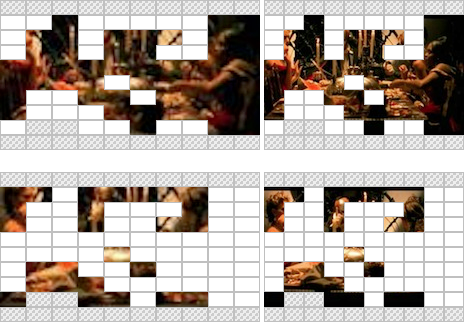
\includegraphics[width=0.75\linewidth]{./similar-different.png}
  \caption{Similar (upper row) and different (lower row) corresponding tile pairs for the media items from a~Facebook (left column) and a~Google+ user (right column); checkerboard tiles are not considered}
  \label{fig:similar-different}
\end{figure}

\begin{figure}[t!]
  \centering
  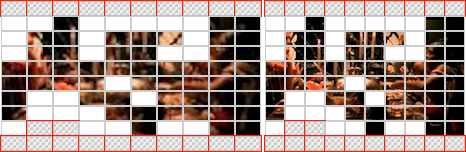
\includegraphics[width=0.8\linewidth]{./tile-highlight.png}
  \caption{Highlighted not considered tiles
    while the text--to--speech system reads the corresponding text fragment
    \textit{``However, 22 tiles were not considered,
    as they are either too bright or too dark,
    which is a common source of clustering issues.''}}
  \label{fig:tile-highlight}
\end{figure}

\section{Evaluation}
\label{sec:evaluation}

For the evaluation of natural language generating systems,
there are three basic techniques.
First, the \emph{task-based} or \emph{extrinsic} evaluation,
where the generated text is given to a~person
who evaluates how well it helps with performing a~given task
(\emph{e.g.},~\cite{portet2009nlg}).
Second, there are \emph{automatic metrics}
(\emph{e.g.}, BLEU~\cite{papineni2002bleu}),
where the generated text is compared to texts written by people
based on the same input data.
Finally, there are \emph{human ratings}, where the generated text
is given to a~person who is asked to rate
the quality and usefulness of the text.

For our evaluation, we chose the third approach of human ratings,
as we do not evaluate the natural language generating system in isolation,
but in \emph{combination with a~visual representation}
that makes use of spatial Media Fragments {\sc uri}s,
as can be seen in \autoref{fig:similar-different}
and \autoref{fig:tile-highlight}.
Evaluating subjective data like the quality and usefulness 
of an auto-generated textual, visual, and audial explanation
of the results of a~deduplication algorithm
is a~challenging task.
For different users, there may be different emphases.
A~common subjective evaluation technique
is the Mean~Opinion Score~(MOS,~\cite{itu1998mos}),
used for decades in telephony networks to
obtain the human user's view of the quality of a~network.
Recently, MOS has also found wider usage in the multimedia community.
Therefore, a~set of standard subjective tests are conducted,
where users rate the perceived quality of test samples
with scores from 1 (worst) to 5 (best).
The actual MOS is then the arithmetic mean of all individual scores.
In the context of this research, we have conducted MOS test sessions
with five external human raters.
We generated artificially modified deduplicated media item sets
around media items about the \emph{Backstreet Boys}
that were shared on social networks during the time of writing.
These media item sets were curated by yet another independent two
external persons, assisted by a~previously developed
software system that implements the deduplication algorithm
described in this paper.
We asked the two persons to provoke dissent and
consent clustering situations for the five human raters,
\emph{i.e.}, obviously correct clustering (\textbf{Clustering Consent}),
obviously incorrect clustering (\textbf{Clustering Dissent}),
and obviously incorrect non-clustering (\textbf{Non-Clustering Dissent}).
We then asked the five human raters to have the system
automatically explain the algorithm results to them
as described in \autoref{sec:from-debug-output-to-story}.
The raters gave MOS scores ranging from $2$ to $5$,
with the overall average values as follows.
\textbf{Clustering Consent}: $4.3$, \textbf{Clustering Dissent}: $3.3$,
and \textbf{Non-Clustering Dissent}: $4.1$.
The human raters appreciated the parallel explanation approach,
where the visual and the audial parts synchronously described
what the algorithm was doing.
They uttered that the due to the black--and--white tolerance
not considered tiles as well as erroneously not detected faces
were sources of error in the algorithm that they easily understood
thanks to the human language description.
They sometimes wished for more diversification in the generated texts,
however, without exception liked the system and encouraged future investment.

\section{Conclusions and Future Work}
\label{sec:conclusions-and-future-work}

% References should be produced using the bibtex program from suitable
% BiBTeX files (here: strings, refs, manuals). The IEEEbib.bst bibliography
% style file from IEEE produces unsorted bibliography list.
% -------------------------------------------------------------------------
\bibliographystyle{IEEEbib}
\bibliography{icme2013template}

\end{document}
